\section{Approach}
% \begin{frame}{Approach}
%     \begin{itemize}
%         \item Data Collection
%         \item Data Augmentation
%         \item Classification Model
%         \item Virtual Environment
%         \item The Framework
%     \end{itemize}
% \end{frame}

\subsection*{Data Collection}
\begin{frame}{Data Collection}
    Data are necessary for the training of the classification models. 
    
    \vspace*{.5cm}
    The data are collected from two datasets: Physionet and Weibo.
    
    \vspace*{.5cm}
    The third one is obtained by considering the common channels and the data points from Physionet.
    \begin{table}[!htbp] 
        \centering 
        \scalebox{.7}[.7]{
            \begin{tabular}{|c|c|c|c|} 
                \hline 
                \textbf{Dataset Name} & \textbf{Number of
    Subjects} & \textbf{Number of Tasks} & \textbf{Number of Channels}\\
                \hline
                \hline 
                Physionet & 109 & 4 & 64\\ 
                \hline 
                Weibo & 10 & 6 & 60\\ 
                \hline 
                \hline
                Reduced Physionet & 109 & 4 & 58\\
                \hline 
            \end{tabular} 
        }
    \end{table}
\end{frame}

\subsection*{Classification Model}
\begin{frame}{Classification Model}
    A classification model is an algorithm that learns to map input data to output labels.

    \vspace*{.5cm}
    Proposed LSTM-based architecture:
    \begin{figure}[!htbp]
        \centering
        \scalebox{0.8}{
        \begin{tikzpicture}[
            squarednode/.style={rectangle, draw=black, very thick, minimum size=5mm},
            ]
            \node[squarednode] (input_data) {Input Data};
            \node[squarednode] (rearrange) [below=of input_data] {Rearrange Data};
            \node[squarednode] (input_layer) [right=of input_data] {Input Layer};
            \node[squarednode] (lstm) [below=of input_layer] {LSTM};
            \node[squarednode] (lstm2) [right=of input_layer] {LSTM};
            \node[squarednode] (output_layer) [right=of lstm] {LSTM Output Filter};
            \node[squarednode] (output) [right=of lstm2] {Output};
            \node[squarednode] (softmax) [right=of output_layer] {Softmax};

            \draw[->] (input_data) -- (rearrange);
            \draw[->] (rearrange) -- (input_layer);
            \draw[->] (input_layer) -- (lstm);
            \draw[->] (lstm) -- (lstm2);
            \draw[->] (lstm2) -- (output_layer);
            \draw[->] (output_layer) -- (output);
            \draw[->] (output) -- (softmax);
        \end{tikzpicture}
        }
    \end{figure}
\end{frame}

\subsection*{Data Augmentation}
\begin{frame}{Data Augmentation}
    Data augmentation is a technique used to increase the size of the dataset by adding noise or generating new data.
    \begin{itemize}
        \item Stochastic Noise Injection
        \item Generative Adversarial Networks (GAN)
    \end{itemize}

    \vspace*{.5cm}
    We used Data Augmentation to test the model on unseen data.
\end{frame}
\begin{frame}{Data Augmentation \textemdash{} Noise Injection}
    \begin{figure}[!htbp]
        \centering
        \begin{tikzpicture}[
            squarednode/.style={rectangle, draw=black, very thick, minimum size=5mm},
            ]
            \node[squarednode] (dataset) {Dataset};
            \node (none3) [right=of dataset] {~};
            \node[squarednode] (sample) [right=of none3] {Sample};
            \node (none) [below=of dataset] {~};
            \node (none2) [below=of sample] {~};
            \node (none4) [below=of none] {~};
            \node (none3) [right=of none4] {~};
            \node[squarednode] (noise) [right=of none3] {Noise};
            \node[squarednode] (plus) [right=of none2] {+};
            \node[squarednode] (output) [right=of plus] {Output};
    
            \draw[->] (dataset) -- node [above] {extract} (sample) ;
            \draw[->] (none4) -- node [above] {generate} (noise) ;
            \draw[->] (sample) -- node [right] {~~add} (plus) ;
            \draw[->] (noise) -- (plus) ;
            \draw[->] (plus) -- (output) ;
        \end{tikzpicture}
    \end{figure}
\end{frame}

\begin{frame}{Data Augmentation \textemdash{} GAN}
    \begin{figure}[!htbp]
        \centering
        \scalebox{0.8}{
        \begin{tikzpicture}[
            squarednode/.style={rectangle, draw=black, very thick, minimum size=5mm},
            ]
            \node[squarednode] (noise) {Noise};
            \node[squarednode] (generator) [right=of noise] {Generator};
            \node[squarednode] (fake_data) [right=of generator] {Fake Data};
            \node (none) [above=of fake_data] {~};
            \node[squarednode] (real_data) [above=of none] {Real Data};
            \node[squarednode] (discriminator) [right=of none] {Discriminator};
            \node[squarednode, dashed] (loss) [right=of discriminator] {Loss};

            \draw[->] (noise) -- (generator);
            \draw[->] (generator) -- (fake_data);
            \draw[->] (real_data) -- (discriminator);
            \draw[->] (fake_data) -- (discriminator);
            \draw[dashed, ->] (discriminator) -- (loss);
            \draw[dashed, ->] (loss) to[out=-90, in=-90] (generator);
            \draw[dashed, ->] (loss) to[out=90, in=90] (discriminator);
        \end{tikzpicture}
        }
    \end{figure}
\end{frame}


\subsection*{Virtual Environment}
\begin{frame}{Virtual Environment}
    A Virtual Environment is a simulated environment that represents a specific scenario or aspect of the real world.

    \vspace*{.5cm}
    To avoid the need for a physical device, such as proshtetic limbs or wheelchairs, we used a virtual environment in which we can test the classification model.

    \vspace*{.5cm}
    \begin{itemize}
        \item \textbf{Unity Engine}: User Friendliness, Development Speed and Portability
        \item Ease of \textbf{Pipeline Test}
    \end{itemize}
\end{frame}
\begin{frame}{Virtual Environment~\textemdash{}~Infinite Runner}
    \begin{minipage}[c]{.49\textwidth}
        \begin{itemize}
            \item \textbf{Constraints}: Automatic Forward (Run) Movement
            \item \textbf{Freedom of Movement}: Jumping, Turning Left and Turning Right
            \item \textbf{Objective}: Avoiding Obstacles, Collecting Coins
        \end{itemize}
    \end{minipage}
    \begin{minipage}[c]{.49\textwidth}
        \begin{figure}
            \centering
            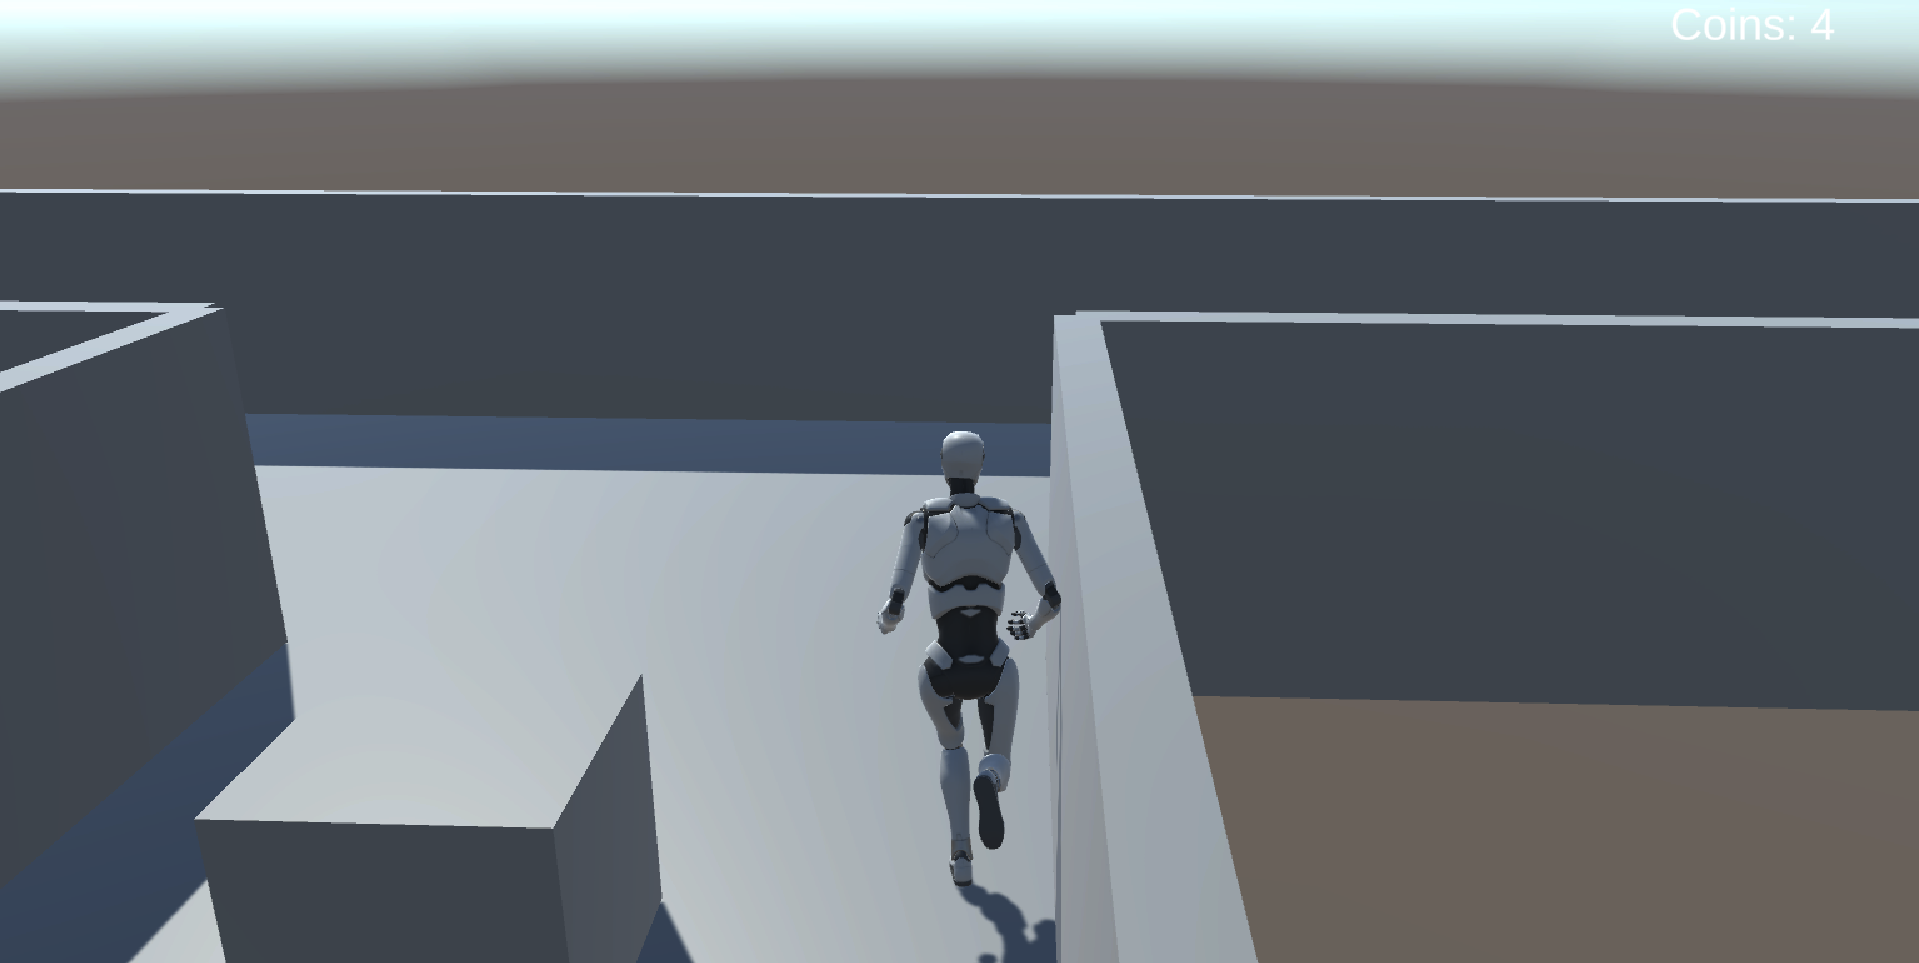
\includegraphics[width=\textwidth]{figures/Methodology/infinite_runner}
        \end{figure}
    \end{minipage}
\end{frame}
\begin{frame}{Virtual Environment~\textemdash{}~Maze Walker}
    \begin{minipage}[c]{.49\textwidth}
        \begin{itemize}
            \item \textbf{Constraints}: Automatic Movememnt (Walk) after direction choice
            \item \textbf{Freedom of Movement}: Forward, Turning Left and Turning Right
            \item \textbf{Objective}: Collecting Coins
        \end{itemize}    
    \end{minipage}
    \begin{minipage}[c]{.49\textwidth}
        \begin{figure}
            \centering
            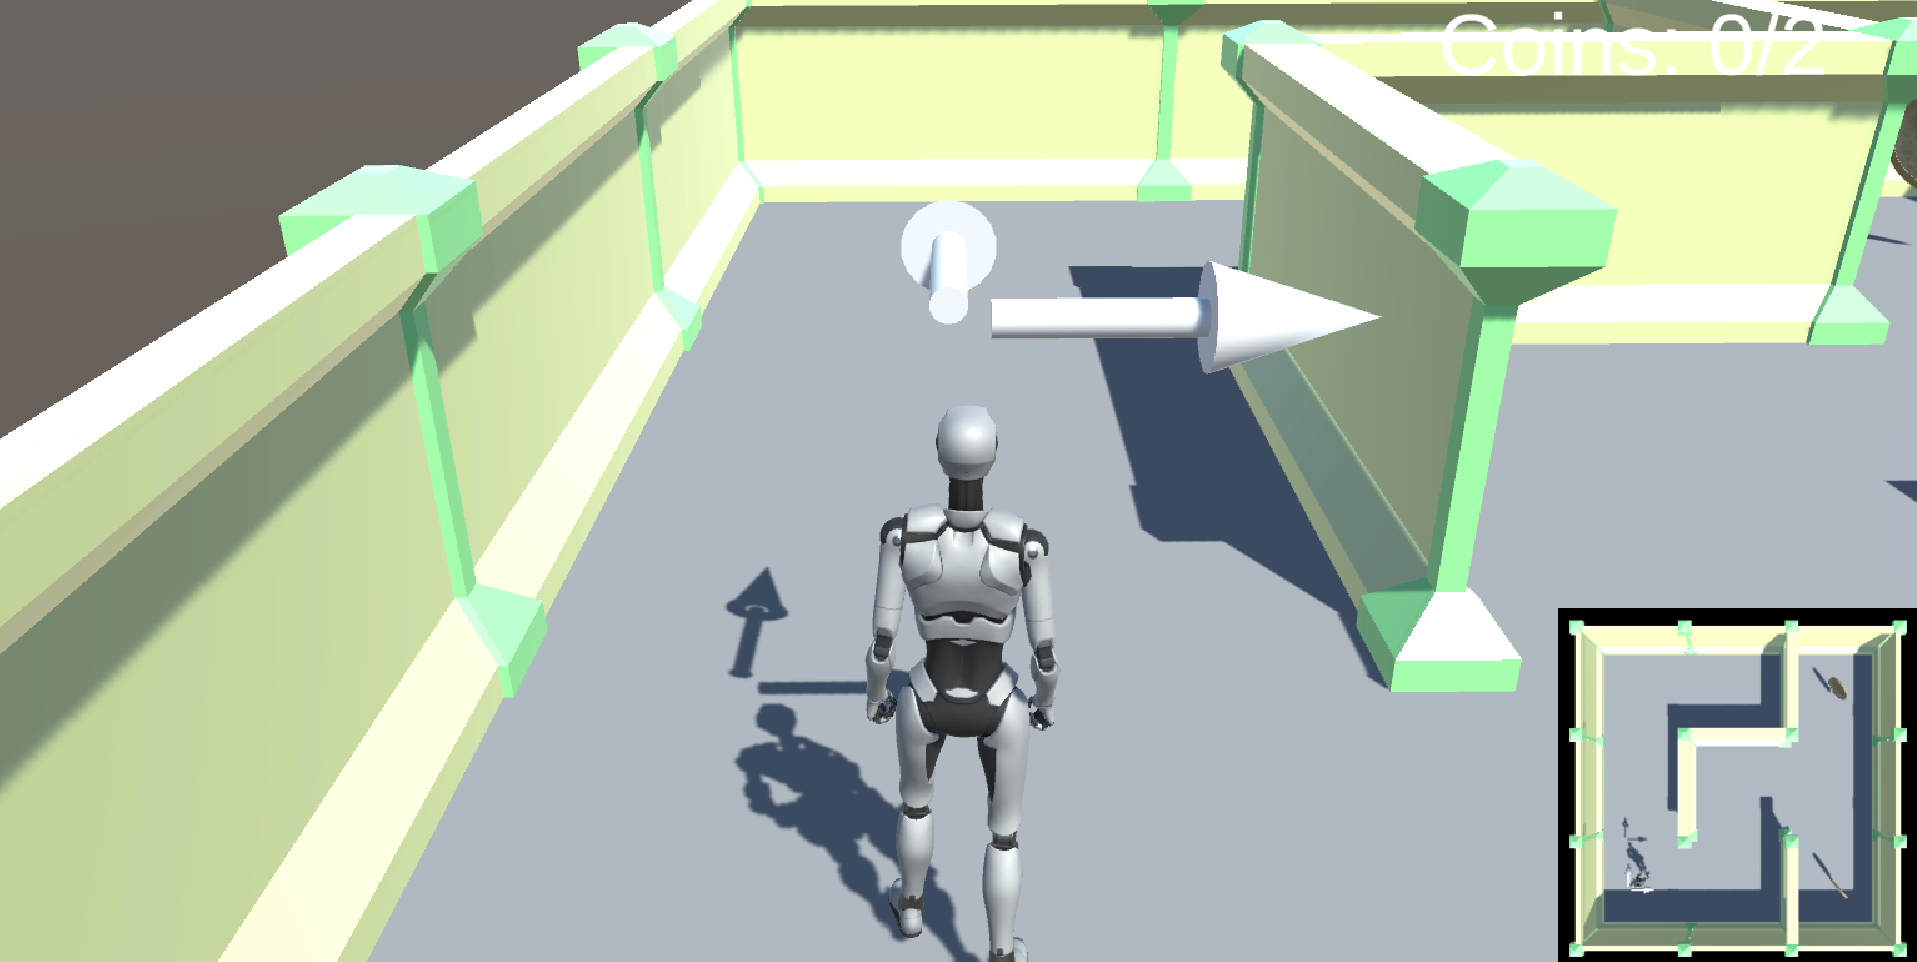
\includegraphics[width=\textwidth]{figures/Methodology/maze}
        \end{figure}
    \end{minipage}
\end{frame}

\subsection*{Full Framework}
\begin{frame}{Full Framework}
    \begin{figure}[!htbp]
        \centering
        \scalebox{0.9}{
        \begin{tikzpicture}[
            squarednode/.style={rectangle, draw=black, very thick, minimum size=5mm},
            ]
            \node[squarednode, dashed] (key_input) {
                \begin{tikzpicture}[
                    squarednode/.style={rectangle, draw=black, very thick, minimum size=5mm},
                    ]
                    \node[squarednode, solid] (keyboard) {Keyboard Input};
                    \node[squarednode, solid] (data_augmentation) [below=of keyboard] {Data Augmentation};
                    
                    \draw[->, solid] (keyboard) -- (data_augmentation);
                \end{tikzpicture}
            };
            \node[] (none) [below=of key_input] {~};
            \node[squarednode, dashed] (EEG_input) [right=of key_input]{
                \begin{tikzpicture}[
                    squarednode/.style={rectangle, draw=black, very thick, minimum size=5mm},
                    ]
                    \node[squarednode, solid] (EEG) {EEG Input};
                    \node[squarednode, solid] (data_filter) [below=of EEG] {Data Filtering};
                    
                    \draw[->, solid] (EEG) -- (data_filter);
                \end{tikzpicture}
            };
            \node[squarednode] (classification) [right=of none] {Classification};
            \node[squarednode] (websocket) [below=of classification] {Websocket};
            \node[squarednode] (virtual_environment) [below=of websocket] {Virtual Environment};

            \draw[->] (key_input) -- (classification);
            \draw[->] (EEG_input) -- (classification);
            \draw[dashed, ->] (classification) -- (websocket);
            \draw[dashed, ->] (websocket) -- (virtual_environment);
        \end{tikzpicture}
        }
    \end{figure}
\end{frame}